\documentclass[tikz]{standalone}

\pagestyle{empty}


\usepackage{amsmath}
\usepackage{tikz}
\usepackage{graphicx}
\usetikzlibrary{positioning,calc,fit,decorations.pathreplacing,arrows,positioning,backgrounds}

% Font settings:
\renewcommand{\familydefault}{\sfdefault}
\usepackage{pxfonts}
\newcommand{\figf}{\sffamily\bfseries\small} %Defines the font used for the labelling of figure panels.


% Color settings:
%\definecolor{hivc}{cmyk}{0,0.80,0.83,0.13}                %\definecolor{hivc}{HTML}{DE2D26}
\definecolor{hivc}{RGB}{24,116,205}
\definecolor{selfc}{cmyk}{0,0,0,0.6}                      %\colorlet{selfc}{gray!80!white}
\definecolor{Rblue}{RGB}{100,149,237}


\begin{document}
\scriptsize

\begin{tikzpicture}[anchor=north west]
	\clip (0,0) rectangle +(18,-7);

	\begin{scope}
		\node[anchor = north west] at (0.1,0) {
			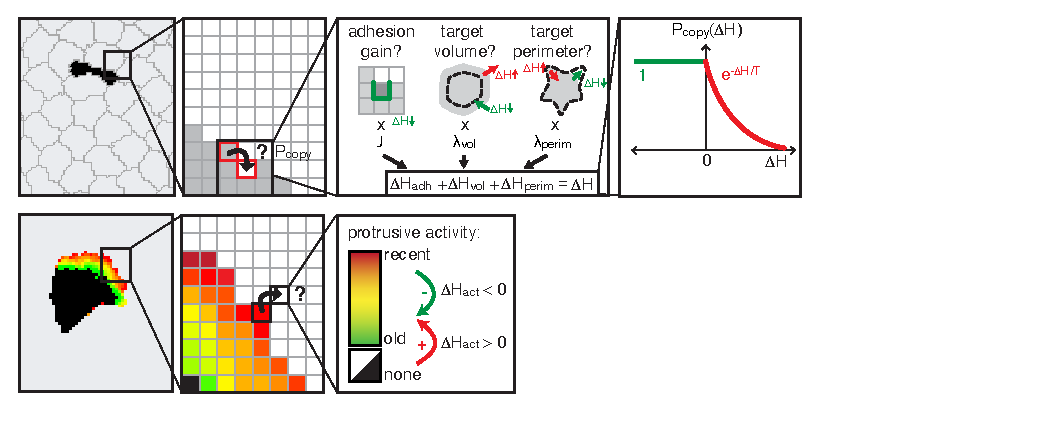
\includegraphics[page=1]{../cartoons/cpm-cartoon.pdf}
		};
		\node[anchor = north west] at (0,0) {\figf A};	
		\node[anchor = north west] at (0,-3.5) {\figf C};
	
	\end{scope}

	\begin{scope}[xshift = 14cm]
		\node[anchor=north west] at (0.55,-0.8) { 
			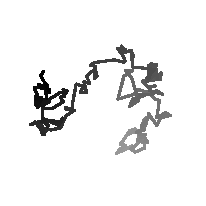
\includegraphics{../twodim/plots/brownian-example-track.pdf}
		};
		\draw[line width = 1pt] (0.4,-0.41) rectangle +(2.1,-1.3);
		\draw[dashed] (0.4,-1.75) -- +(1,-0.35);
		\draw[dashed] (2.5,-1.75) -- +(-1.1,-0.35);
		\node[anchor=north west] at (0.3,-0.3) {
			\includegraphics[page=2]{../cartoons/cpm-cartoon.pdf}
		};
		\node[anchor = north west] at (0,0) {\figf B};	
	\end{scope}

	\begin{scope}[xshift = 9cm,yshift=-3.5cm]
		\node[anchor=north west] at (0.5,-0.3) { 
			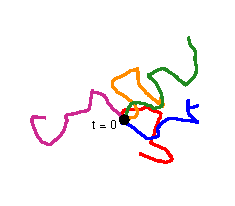
\includegraphics{../twodim/plots/act-example-tracks.pdf}
		};
		\draw[line width = 1pt] (0.4,-0.25) rectangle +(2.1,-1.3);
		\draw[dashed] (2.5,-0.25) -- +(1.3,-0.8);
		\draw[dashed] (2.5,-1.55) -- +(1.3,0.5);
		\node[anchor=north west] at (0.3,-0.15) {
			\includegraphics[page=3]{../cartoons/cpm-cartoon.pdf}
		};
		\node[anchor = north west] at (0,0) {\figf D};	
	\end{scope}

	\begin{scope}[xshift = 13cm,yshift=-3.5cm]
		\node[anchor=north west] at (0,0) { 
			\includegraphics{../twodim/plots/displacement-actVsBrownian.pdf}
		};
		\node[anchor = north west] at (0,0) {\figf E};	
	\end{scope}


\end{tikzpicture}



\end{document}